\chapter{Sintesis Asimetris}\label{ch:b3:asymmetric-synthesis}

L-DOPA, obat yang meringankan gejala penyakit Parkinson, pada tahun
1970-an menjadi senyawa pertama yang dibuat secara industri melalui \omterm{def:b3:asymmetric-synthesis:asymmetric-catalysis}{katalisis asimetris}: beberapa
gram kompleks rodium kiral, yang dilarutkan bersama sebuah prekursor datar yang akiral
di bawah hidrogen, memberikan produk yang salah satu enantiomernya jauh melebihi
enantiomer lainnya. Kedua enantiomer sebuah obat dapat berbeda sama sekali dalam efeknya,
karena reseptor dan \omterm{def:b3:complex-kinetics:enzyme}{enzim} yang dijumpainya sendiri bersifat kiral. Bab ini
mengukur kemurnian enantiomer, menjelaskan bagaimana lingkungan kiral memilih
di antara dua jalur yang saling bayangan cermin, dan membahas strategi-strategi (\omterm{def:b3:asymmetric-synthesis:chiral-pool}{kumpulan kiral},
auksiliari, resolusi, katalis logam dan katalis organik) yang membuat enantiomer
tunggal.

\begin{recall}
Jilid Tahun 1 mendefinisikan kiralitas, enantiomer, diastereomer, campuran
rasemat, rotasi spesifik, aturan CIP, serta reaksi stereoselektif dan
stereospesifik; Jilid Tahun 2 membahas hidrogenasi katalitik,
epoksidasi, dihidroksilasi, imina, enamina, enolat, reaksi aldol,
anulasi Robinson, dan kromatografi. \Cref{ch:b3:rate-theories} memberikan
\omterm{thm:b3:rate-theories:eyring}{persamaan Eyring}, \cref{ch:b3:homogeneous-catalysis} siklus Wilkinson, dan
\cref{ch:b3:point-groups} sumbu $C_2$.
\end{recall}

\begin{omfigure}
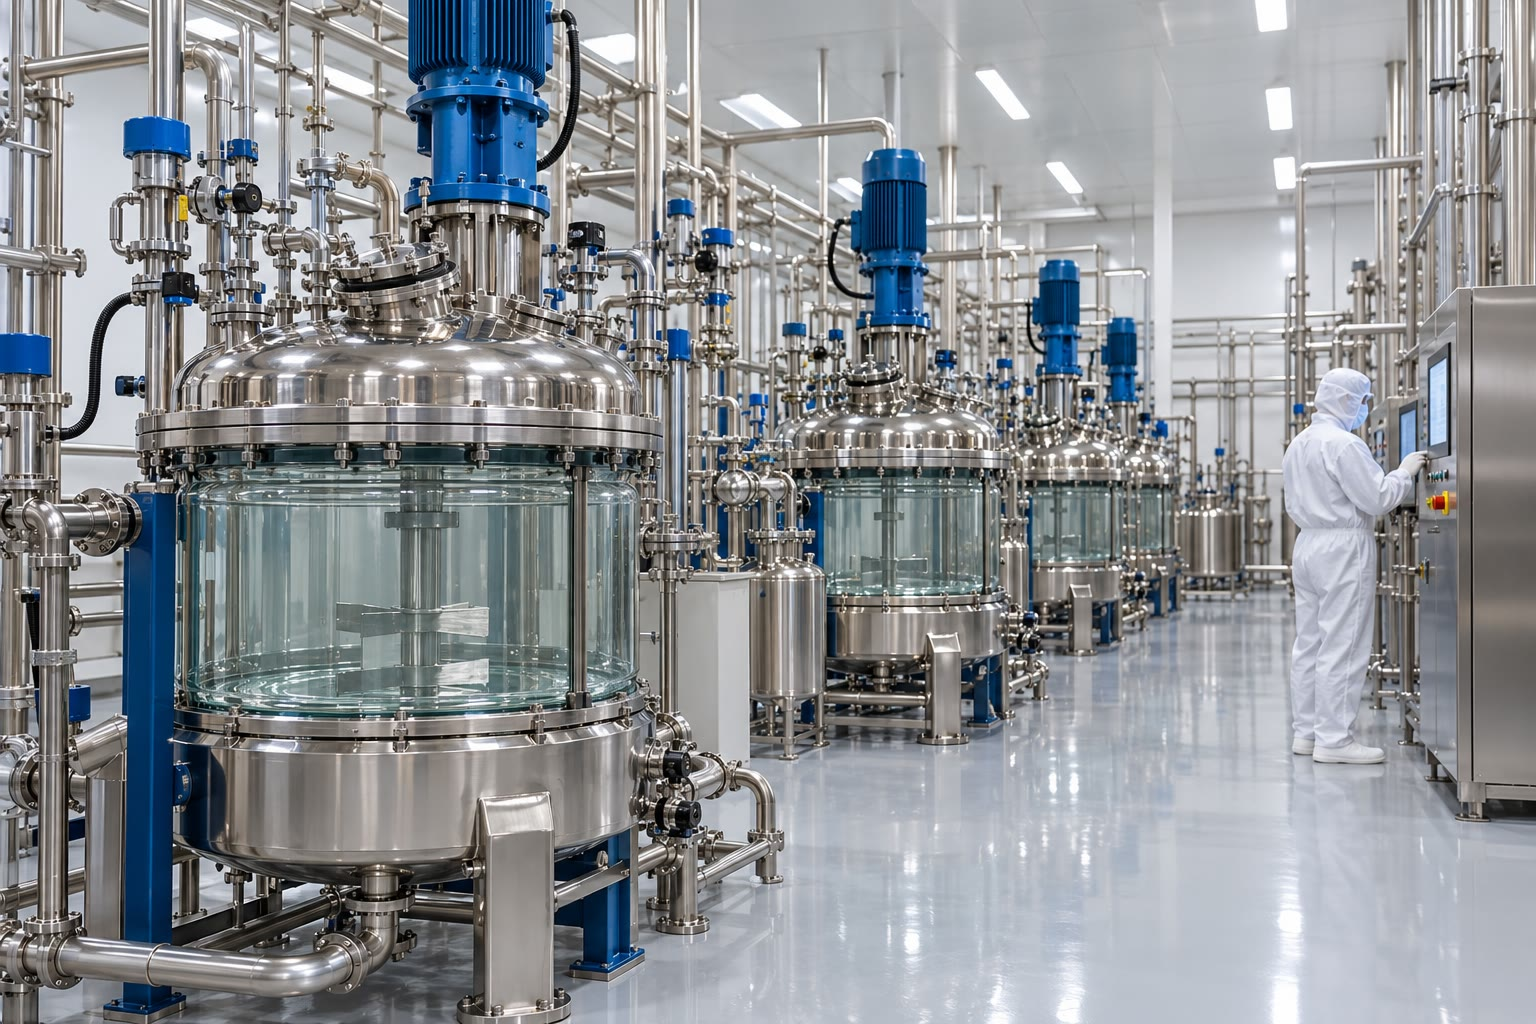
\includegraphics[width=0.58\linewidth]{images/book4/ai/b3-28-api-plant.jpg}

{\small Sebuah aula berisi reaktor berlapis kaca di pabrik yang membuat bahan aktif
farmasi. Banyak produknya berupa enantiomer tunggal, yang dibuat
melalui katalisis atau resolusi dan diperiksa dengan kromatografi kiral.}
\end{omfigure}

\section{Mengukur kemurnian enantiomer}

\begin{definition}[Kelebihan enantiomer]\label{def:b3:asymmetric-synthesis:ee}
Untuk campuran enantiomer dalam jumlah $n_R \ge n_S$, yang disebut \emph{kelebihan
enantiomer}\index{kelebihan enantiomer} adalah $\mathrm{ee} = (n_R - n_S)/(n_R + n_S)$ dan \emph{rasio enantiomer}
\index{rasio enantiomer} adalah $\mathrm{er} = n_R/n_S$; untuk diastereomer, \emph{kelebihan
diastereomer}\index{kelebihan diastereomer}, de, didefinisikan dengan cara yang
sama. Yang disebut \emph{kemurnian optis}\index{kemurnian optis} adalah rasio
rotasi spesifik sebuah sampel terhadap rotasi spesifik enantiomer murninya.
\end{definition}

\begin{proposition}[ee dan er]\label{prop:b3:asymmetric-synthesis:ee-er}
$\mathrm{ee} = (\mathrm{er} - 1)/(\mathrm{er} + 1)$ dan $\mathrm{er} = (1 + \mathrm{ee})/(1 - \mathrm{ee})$.
\end{proposition}

\begin{proof}
Bagilah pembilang dan penyebut $(n_R - n_S)/(n_R + n_S)$ dengan $n_S$; menyelesaikannya untuk er memberikan
bentuk kedua.
\end{proof}

ee sebesar 90\,\% adalah er 95\,:\,5, dan ee 98\,\% adalah er 99\,:\,1. \omterm{def:b3:asymmetric-synthesis:ee}{Kemurnian optis}
sama dengan ee hanya jika rotasi sebanding dengan komposisi; pengotor,
pelarut, efek konsentrasi, dan rotasi yang kecil pada banyak senyawa membuatnya
tidak andal, sehingga ee diukur dengan memisahkan enantiomer-enantiomernya.

\begin{method}[ee dari kromatogram kiral]\label{met:b3:asymmetric-synthesis:ee-chromatogram}
\begin{enumerate}
  \item Injeksikan rasematnya lebih dahulu, untuk mengenali kedua puncak dan memeriksa
        pemisahannya (resolusi sampai garis dasar) serta luasnya yang sama.
  \item Injeksikan sampelnya dan integrasikan kedua puncak.
  \item Enantiomer-enantiomer memberikan respons yang sama pada detektor akiral, sehingga
        $\mathrm{ee} = (A_1 - A_2)/(A_1 + A_2)$; tetapkan puncak-puncaknya dengan standar yang murni enantiomer.
\end{enumerate}
\end{method}

\begin{omfigure}
\begin{tikzpicture}
\begin{axis}[name=a, width=0.48\linewidth, height=5.4cm, xmin=0, xmax=20, ymin=0, ymax=1.0,
  axis lines=left, xlabel={$\Delta\Delta G^\ddagger$ / \unit{kJ.mol^{-1}}}, ylabel={ee},
  tick label style={font=\scriptsize}, label style={font=\small}]
\addplot[omDef, thick] table[x=ddg, y=eeA] {figdata/out/bachelor-3-er-ddg.dat};
\addplot[omMeth, thick] table[x=ddg, y=eeB] {figdata/out/bachelor-3-er-ddg.dat};
\addplot[omThm, thick] table[x=ddg, y=eeC] {figdata/out/bachelor-3-er-ddg.dat};
\node[font=\scriptsize, omDef, anchor=west] at (axis cs:10,0.55) {\qty{-78}{\celsius}};
\node[font=\scriptsize, omMeth, anchor=west] at (axis cs:10,0.43) {\qty{0}{\celsius}};
\node[font=\scriptsize, omThm, anchor=west] at (axis cs:10,0.31) {\qty{25}{\celsius} (kurva terbawah)};
\end{axis}
\begin{axis}[at={(a.east)}, anchor=west, xshift=1.4cm, width=0.48\linewidth, height=5.4cm,
  xmin=7.5, xmax=9.5, ymin=0, axis lines=left, ytick=\empty,
  xlabel={waktu retensi / min}, ylabel={sinyal detektor},
  tick label style={font=\scriptsize}, label style={font=\small}]
\addplot[black, thick] table[x=t, y=y] {figdata/out/bachelor-3-er-ddg-b.dat};
\node[font=\scriptsize, anchor=south west] at (axis cs:8.3,250) {(\textit{R}): 97.5};
\node[font=\scriptsize, anchor=south] at (axis cs:9.1,20) {(\textit{S}): 2.5};
\end{axis}
\end{tikzpicture}

{\small Kiri: \omterm{def:b3:asymmetric-synthesis:ee}{kelebihan enantiomer} terhadap selisih \omterm{def:b3:rate-theories:activation}{energi Gibbs
aktivasi} kedua jalur yang bersaing, pada tiga suhu: $\Delta\Delta G^\ddagger$ yang
sama memberikan ee yang lebih tinggi pada suhu rendah. Kanan: kromatogram HPLC kiral,
luas puncak 97.5 dan 2.5 (model): ee 95\,\%.}
\end{omfigure}

NMR membedakan enantiomer hanya dalam lingkungan kiral: zat pelarut kiral
membentuk kompleks diastereomer berumur pendek yang sinyalnya berbeda, dan
alkohol atau amina kiral yang diubah menjadi kedua ester diastereomernya dengan
asam Mosher memperlihatkan konfigurasinya dari pola selisih geseran.

\begin{method}[Konfigurasi dari ester Mosher, secara garis besar]\label{met:b3:asymmetric-synthesis:mosher}
\begin{enumerate}
  \item Buatlah ester MTPA (\textit{R}) dan (\textit{S}) alkohol itu.
  \item Rekamlah spektrum protonnya dan hitunglah $\Delta\delta = \delta_S - \delta_R$ untuk proton-proton di setiap
        sisi karbon karbinol.
  \item Dalam konformasi yang disukai, cincin fenil asam itu melindungi satu sisi:
        proton dengan $\Delta\delta > 0$ terletak di satu sisi, proton dengan $\Delta\delta < 0$ di sisi lain, yang
        menempatkan kedua substituen dan memberikan konfigurasinya.
\end{enumerate}
\end{method}

\section{Topisitas dan adisi stereoselektif}

\begin{definition}[Reaksi stereoselektif]\label{def:b3:asymmetric-synthesis:selective}
Yang disebut \emph{reaksi enantioselektif}\index{reaksi enantioselektif} adalah reaksi yang membentuk satu
enantiomer produk secara berlebih dibandingkan dengan enantiomer lainnya; sedangkan \emph{reaksi
diastereoselektif}\index{reaksi diastereoselektif} membentuk satu diastereomer secara berlebih.
\end{definition}

\begin{definition}[Topisitas]\label{def:b3:asymmetric-synthesis:topicity}
Dua gugus dalam sebuah molekul disebut \emph{homotopik}\index{homotopik} jika dipertukarkan oleh
rotasi molekul (mengganti salah satunya memberikan senyawa yang sama),
\emph{enantiotopik}\index{enantiotopik} jika hanya dipertukarkan oleh refleksi
(mengganti yang satu atau yang lain memberikan enantiomer), dan
\emph{diastereotopik}\index{diastereotopik} jika tidak ada \omterm{def:b3:point-groups:operation}{operasi simetri} yang mempertukarkannya
(mengganti yang satu atau yang lain memberikan diastereomer).
\end{definition}

Kedua hidrogen gugus $\ce{CH2}$ di samping sebuah pusat stereo bersifat \omterm{def:b3:asymmetric-synthesis:topicity}{diastereotopik}: keduanya
memiliki geseran kimia yang berbeda dan saling berkopling, dan itulah sebabnya gugus semacam itu
sering tampak sebagai dua sinyal dalam NMR.

\begin{definition}[Muka prokiral]\label{def:b3:asymmetric-synthesis:faces}
Karbon trigonal dengan tiga substituen yang berbeda bersifat \emph{prokiral}\index{prokiral}:
adisi gugus keempat yang berbeda menciptakan pusat stereo. Mukanya yang dilihat dengan
ketiga substituen menurut prioritas CIP yang menurun berurutan searah jarum jam disebut
\emph{muka Re}\index{muka Re}; jika berlawanan arah jarum jam, \emph{muka Si}\index{muka Si}.
\end{definition}

\begin{omfigure}
\begin{tikzpicture}[font=\small, >=Stealth]
  \coordinate (c) at (0,0);
  \draw[thick, double, double distance=1.6pt] (c) -- (90:1.1) node[above] {O (1)};
  \draw[thick] (c) -- (210:1.1) node[below left] {$\ce{C6H5}$ (2)};
  \draw[thick] (c) -- (330:1.1) node[below right] {$\ce{CH3}$ (3)};
  \fill (c) circle (1.6pt);
  \draw[->, thick, omThm] (70:0.6) arc[start angle=70, end angle=200, radius=0.6];
  \node[font=\scriptsize, omThm, align=center] at (-2.2,0.75) {1 $\to$ 2 $\to$ 3\\ berlawanan arah\\ jarum jam: muka \textit{Si}};
  \node[font=\scriptsize, align=left, anchor=west] at (2.6,0.4) {muka yang menghadap pembaca: \textit{Si}\\ muka di balik halaman: \textit{Re}};
  \node[font=\scriptsize, align=left, anchor=west] at (2.6,-0.5) {hidrida yang ditambahkan dari muka \textit{Re}\\ memberikan (\textit{S})-1-feniletanol};
\end{tikzpicture}

{\small Muka-muka asetofenon. Dilihat dari depan, substituen-substituen
karbon karbonil menurut urutan CIP (O, fenil, metil) berurutan berlawanan arah jarum jam: muka
depan adalah \textit{Si}, muka belakang \textit{Re}.}
\end{omfigure}

\begin{method}[Menetapkan muka Re dan Si]\label{met:b3:asymmetric-synthesis:re-si}
\begin{enumerate}
  \item Urutkan ketiga substituen atom trigonal itu menurut aturan CIP (ikatan
        rangkap menghitung pasangannya dua kali).
  \item Lihatlah muka yang ditinjau, dengan bidang trigonal pada bidang halaman.
  \item Searah jarum jam 1 $\to$ 2 $\to$ 3: \textit{Re}; berlawanan arah jarum jam: \textit{Si}.
  \item Untuk menamai produknya, tambahkan gugus baru ke arah pengamat dan terapkan
        aturan CIP pada pusat stereo yang baru; serangan Re tidak selalu memberikan \textit{R}.
\end{enumerate}
\end{method}

\begin{definition}[Model Felkin--Anh dan kendali kelasi]\label{def:b3:asymmetric-synthesis:felkin}
Yang disebut \emph{model Felkin--Anh}\index{model Felkin--Anh} adalah model yang meramalkan
diastereomer utama adisi nukleofilik pada gugus karbonil yang bersebelahan dengan sebuah
pusat stereo: gugus terbesar pada pusat itu terletak tegak lurus terhadap bidang
karbonil, dan nukleofil mendekat secara anti terhadapnya, melewati gugus
terkecil, sepanjang lintasan Bürgi--Dunitz. Di bawah \emph{kendali
kelasi}\index{kendali kelasi}, ion logam yang terikat sekaligus pada oksigen karbonil
dan pada gugus donor di pusat stereo mengunci konformasinya, dan
nukleofil teradisi pada muka cincin kelat yang kurang terhalang.
\end{definition}

\begin{proposition}[Selektivitas Felkin--Anh]\label{prop:b3:asymmetric-synthesis:felkin}
Untuk aldehida atau keton yang kiral di posisi $\alpha$ tanpa gugus pengelat, produk
utamanya adalah produk yang diramalkan \omterm{def:b3:asymmetric-synthesis:felkin}{model Felkin--Anh} (sebuah model empiris,
yang didukung perhitungan). \admitted
\end{proposition}

\begin{omfigure}
\begin{tikzpicture}[font=\small, >=Stealth]
  \foreach \a/\lab in {90/L, 330/M, 210/S} {
    \draw[line width=0.8pt] (\a:0.55) -- (\a:1.1) node[pos=1.3] {\lab};
  }
  \fill[white] (0,0) circle (0.55);
  \draw[line width=0.8pt] (0,0) circle (0.55);
  \draw[line width=0.8pt, double, double distance=1.4pt] (0,0) -- (0:1.1) node[right] {O};
  \draw[line width=0.8pt] (0,0) -- (180:1.1) node[left] {R};
  \draw[->, very thick, omThm] (250:2.2) -- (250:0.25);
  \node[omThm, anchor=north] at (250:2.25) {Nu$^-$};
  \node[font=\scriptsize, align=left, anchor=west] at (1.7,-1.0) {Nu$^-$ masuk anti terhadap L,\\ melewati S, pada sekitar 107°\\ terhadap ikatan C=O};
\end{tikzpicture}

{\small \omterm{def:b3:asymmetric-synthesis:felkin}{Model Felkin--Anh}, dilihat sepanjang ikatan dari karbon karbonil (depan,
ikatan ke O dan R) ke pusat stereo (lingkaran belakang, gugus L, M, dan S). Gugus
besar tegak lurus terhadap bidang karbonil; nukleofil datang dari
sisi yang berlawanan, dekat dengan gugus kecil dan jauh dari oksigen.}
\end{omfigure}

\section{Strategi}

\begin{definition}[Kumpulan kiral]\label{def:b3:asymmetric-synthesis:chiral-pool}
Yang disebut \emph{kumpulan kiral}\index{kumpulan kiral} adalah himpunan senyawa alam yang murah dan
murni enantiomer (asam amino, gula, terpena, asam hidroksi) yang dipakai sebagai
bahan awal, dengan pusat-pusat stereonya terbawa ke dalam target.
\end{definition}

\begin{definition}[Auksiliari kiral]\label{def:b3:asymmetric-synthesis:auxiliary}
Yang disebut \emph{auksiliari kiral}\index{auksiliari kiral} adalah gugus murni enantiomer yang
dipasang sementara pada substrat untuk mengendalikan stereokimia sebuah
reaksi, lalu dilepaskan dan diperoleh kembali.
\end{definition}

Dalam alkilasi Evans, sebuah oksazolidinon yang dibuat dari asam amino diasilasi;
enolat litium atau natriumnya, yang terkelat pada gugus karbonil auksiliari itu,
diserang oleh alkil halida pada muka yang jauh dari substituen auksiliari,
sehingga terbentuk satu diastereomer, sering dengan de di atas 95\,\%; hidrolisis lalu membebaskan
asam kiral itu dan auksiliarinya.

\begin{definition}[Resolusi]\label{def:b3:asymmetric-synthesis:resolution}
Yang disebut \emph{resolusi rasemat}\index{resolusi rasemat} adalah
pemisahannya menjadi enantiomer-enantiomer, secara klasik dengan mengkristalkan garam diastereomer
dengan asam atau basa murni enantiomer. Dalam \emph{resolusi kinetik}\index{resolusi kinetik},
kedua enantiomer bereaksi dengan laju yang berbeda dengan pereaksi atau
katalis kiral, dengan selektivitas $s = k_{\mathrm{fast}}/k_{\mathrm{slow}}$. Dalam \emph{resolusi kinetik
dinamis}\index{resolusi kinetik dinamis}, enantiomer-enantiomer substrat
saling berubah dengan cepat sementara salah satunya bereaksi.
\end{definition}

\begin{theorem}[Persamaan Kagan]\label{thm:b3:asymmetric-synthesis:kagan}
Dalam \omterm{def:b3:asymmetric-synthesis:resolution}{resolusi kinetik} sebuah rasemat melalui reaksi-reaksi orde satu dengan selektivitas $s$,
konversi $c$ dan ee substrat yang tersisa dihubungkan oleh
\[
  s = \frac{\ln[(1 - c)(1 - \mathrm{ee})]}{\ln[(1 - c)(1 + \mathrm{ee})]}.
\]
\end{theorem}

\begin{proof}
Setiap enantiomer meluruh secara eksponensial: fraksi yang tersisa adalah $f_1 = \eu^{-k_{\mathrm{fast}}t}$ dan
$f_2 = \eu^{-k_{\mathrm{slow}}t}$, sehingga $\ln f_1 = s\ln f_2$. Mulai dari jumlah yang sama, $1 - c = (f_1 + f_2)/2$ dan
$\mathrm{ee} = (f_2 - f_1)/(f_1 + f_2)$. Maka $(1 - c)(1 - \mathrm{ee}) = \tfrac12(f_1 + f_2)\cdot 2f_1/(f_1 + f_2) = f_1$ dan dengan cara yang sama
$(1 - c)(1 + \mathrm{ee}) = f_2$. Jadi $s = \ln f_1/\ln f_2$ adalah rasio yang dinyatakan.
\end{proof}

\begin{omfigure}
\begin{tikzpicture}
\begin{axis}[width=0.62\linewidth, height=5.6cm, xmin=0, xmax=1, ymin=0, ymax=1.02,
  axis lines=left, xlabel={konversi $c$}, ylabel={ee},
  tick label style={font=\scriptsize}, label style={font=\small},
  legend style={font=\scriptsize, draw=none, at={(1.04,0.5)}, anchor=west}, legend cell align=left]
\addplot[color=omThm, thick] table[x=c, y=eesm] {figdata/out/bachelor-3-kinetic-resolution-s2.dat};
\addlegendentry{$s = 2$}
\addplot[color=omMeth, thick] table[x=c, y=eesm] {figdata/out/bachelor-3-kinetic-resolution-s10.dat};
\addlegendentry{$s = 10$}
\addplot[color=omDef, thick] table[x=c, y=eesm] {figdata/out/bachelor-3-kinetic-resolution-s50.dat};
\addlegendentry{$s = 50$}
\addplot[color=omThm, thick, dashed] table[x=c, y=eep] {figdata/out/bachelor-3-kinetic-resolution-s2.dat};
\addplot[color=omMeth, thick, dashed] table[x=c, y=eep] {figdata/out/bachelor-3-kinetic-resolution-s10.dat};
\addplot[color=omDef, thick, dashed] table[x=c, y=eep] {figdata/out/bachelor-3-kinetic-resolution-s50.dat};
\end{axis}
\end{tikzpicture}

{\small \omterm{def:b3:asymmetric-synthesis:resolution}{Resolusi kinetik}: ee substrat yang tersisa (garis utuh) dan
produk (putus-putus) terhadap konversi, untuk tiga selektivitas. Substrat
selalu dapat dibuat murni enantiomer dengan melanjutkan reaksi cukup jauh, dengan mengorbankan rendemen;
produk paling murni pada konversi rendah.}
\end{omfigure}

\begin{proposition}[Resolusi kinetik dinamis]\label{prop:b3:asymmetric-synthesis:dkr}
Jika enantiomer-enantiomer substrat saling berubah jauh lebih cepat daripada laju reaksi masing-masing,
seluruh rasemat dapat diubah menjadi satu enantiomer produk, dengan ee yang ditentukan oleh $s$:
$\mathrm{er} = s$.
\end{proposition}

\begin{proof}
Rasemisasi yang cepat menjaga kedua enantiomer substrat dalam jumlah yang sama setiap
saat. Produk-produk lalu terbentuk dengan laju yang perbandingannya $k_{\mathrm{fast}}[\mathrm A] : k_{\mathrm{slow}}[\mathrm A] = s$, dan tidak ada yang
menghentikan reaksi sebelum seluruh substrat, sebagian besar melalui enantiomer yang cepat,
habis terpakai: rendemennya dapat mencapai 100\,\% dengan $\mathrm{er} = s$.
\end{proof}

\begin{method}[Memilih strategi]\label{met:b3:asymmetric-synthesis:strategy}
\begin{enumerate}
  \item Jika pusat-pusat stereo target terdapat dalam senyawa alam yang murah, mulailah
        dari \omterm{def:b3:asymmetric-synthesis:chiral-pool}{kumpulan kiral}.
  \item Untuk sintesis sekali jalan, atau untuk menetapkan sebuah pusat secara andal di samping gugus
        karbonil, pakailah auksiliari, dengan biaya dua tahap tambahan.
  \item Jika rasematnya murah dan enantiomer yang tidak dikehendaki dapat didaur ulang atau
        dirasemisasi, resolusikan rasemat itu (secara klasik, kinetik, atau dinamis).
  \item Untuk skala besar, carilah katalis asimetris: satu pusat stereo dibuat
        per perputaran katalitik, tanpa limbah kiral stoikiometrik.
\end{enumerate}
\end{method}

\section{Katalisis asimetris dengan logam}

\begin{definition}[Katalisis asimetris]\label{def:b3:asymmetric-synthesis:asymmetric-catalysis}
Yang disebut \emph{katalisis asimetris}\index{katalisis asimetris} adalah sintesis
enantioselektif dengan katalis kiral yang dipakai dalam jumlah kecil; untuk katalis logam,
kiralitasnya biasanya berasal dari \emph{ligan kiral}\index{ligan kiral}.
\end{definition}

\begin{theorem}[Selektivitas dari energi]\label{thm:b3:asymmetric-synthesis:er-ddg}
Jika dua produk enantiomer terbentuk melalui keadaan transisi diastereomer
dengan faktor praeksponensial yang sama, secara ireversibel, di bawah kendali kinetika,
$\mathrm{er} = \exp(\Delta\Delta G^\ddagger/RT)$, dengan $\Delta\Delta G^\ddagger$ selisih \omterm{def:b3:rate-theories:activation}{energi Gibbs
aktivasi} keduanya.
\end{theorem}

\begin{proof}
Menurut \omterm{thm:b3:rate-theories:eyring}{persamaan Eyring} (\cref{ch:b3:rate-theories}),
$k_i = (k_BT/h)\eu^{-\Delta G_i^\ddagger/RT}$; kedua produk terbentuk dari pereaksi yang sama, sehingga pada setiap saat
lajunya berbanding $k_1/k_2 = \eu^{(\Delta G_2^\ddagger - \Delta G_1^\ddagger)/RT}$, demikian pula jumlah yang terbentuk.
\end{proof}

Pada \qty{25}{\celsius}, ee sebesar 99\,\% (er 199) memerlukan $\Delta\Delta G^\ddagger = RT\ln 199 = \qty{13.1}{kJ/mol}$, kira-kira energi
satu ikatan hidrogen; pada \qty{-78}{\celsius}, \qty{8.6}{kJ/mol} sudah cukup.

\begin{proposition}[Ligan bersimetri $C_2$]\label{prop:b3:asymmetric-synthesis:c2}
\omterm{def:b3:asymmetric-synthesis:asymmetric-catalysis}{Ligan kiral} bersimetri $C_2$ mengurangi menjadi setengah jumlah keadaan transisi
diastereomer yang harus dibandingkan, karena kedua situs koordinasi yang disisakannya
setara.
\end{proposition}

\begin{proof}
Rotasi $C_2$ katalis memetakan satu situs bebas ke situs yang lain dan membiarkan
katalis tidak berubah; karena itu setiap keadaan transisi pada satu situs identik dengan
keadaan transisi terputar pada situs yang lain. Hanya modus-modus pengikatan pada satu situs (muka substrat,
orientasi) yang perlu dibandingkan.
\end{proof}

Knowles memakai monofosfina kiral, lalu difosfina bersimetri $C_2$ DIPAMP, bersama rodium untuk
menghidrogenasi sebuah enamida menjadi asam amino terlindung L-DOPA; BINAP Noyori,
bersama rutenium, menghidrogenasi keton dan alkena terfungsionalisasi, dan,
jika dipadukan dengan diamina kiral, keton sederhana dengan ee yang sangat tinggi. Dalam
hidrogenasi enamida dengan rodium, produk utama berasal dari kompleks katalis--substrat minor
yang kurang stabil, yang bereaksi jauh lebih cepat dengan hidrogen:
selektivitas ditentukan pada keadaan transisi, bukan oleh \omterm{def:b3:partition-functions:boltzmann}{populasi}
zat-zat antara (asas Curtin--Hammett).

\begin{definition}[Epoksidasi Sharpless]\label{def:b3:asymmetric-synthesis:sharpless}
Yang disebut \emph{epoksidasi Sharpless}\index{epoksidasi Sharpless} adalah
epoksidasi enantioselektif alkohol alilik oleh \textit{tert}-butil hidroperoksida,
yang dikatalisis oleh titanium(IV) isopropoksida dengan dietil tartrat yang murni enantiomer;
alkohol itu terikat pada titanium, yang mengantarkan oksigen ke satu muka
alkena, yang dipilih oleh tartrat itu.
\end{definition}

\begin{omfigure}
\begin{tikzpicture}[font=\small, >=Stealth]
  \draw[black!50] (-2.3,-1.55) rectangle (2.5,1.55);
  % C3 (atas) = C2 (bawah); C2 membawa R1 (kiri) dan CH2OH (kanan bawah),
  % C3 membawa R2 (kiri) dan R3 (kanan)
  \coordinate (c3) at (0,0.45); \coordinate (c2) at (0,-0.45);
  \draw[thick, double, double distance=1.6pt] (c3) -- (c2);
  \draw[thick] (c3) -- (-0.9,0.95) node[above left, inner sep=1pt] {R$^2$};
  \draw[thick] (c3) -- (0.9,0.95) node[above right, inner sep=1pt] {R$^3$};
  \draw[thick] (c2) -- (-0.9,-0.95) node[below left, inner sep=1pt] {R$^1$};
  \draw[thick] (c2) -- (0.9,-0.95) node[below right, inner sep=1pt] {$\ce{CH2OH}$};
  \draw[->, very thick, omDef] (0.35,2.5) -- (0.2,0.1) node[pos=0, above, align=center, font=\scriptsize] {D-($-$)-dietil tartrat:\\ O dari muka atas};
  \draw[->, very thick, omThm] (0.35,-2.6) -- (0.2,-0.1) node[pos=0, below, align=center, font=\scriptsize] {L-($+$)-dietil tartrat:\\ O dari muka bawah};
\end{tikzpicture}

{\small Jembatan keledai Sharpless. Dengan alkohol alilik yang digambar pada bidang, dan
gugus $\ce{CH2OH}$ di kanan bawah, L-($+$)-dietil tartrat mengantarkan oksigen dari
bawah bidang dan D-($-$)-dietil tartrat dari atas, apa pun
substituen $\mathrm R^1$ sampai $\mathrm R^3$-nya.}
\end{omfigure}

Gagasan yang sama, yaitu logam yang dipegang dalam kantong kiral oleh ligan alam yang murah, memberikan
dihidroksilasi asimetris Sharpless untuk alkena dengan osmium dan ligan alkaloid
kina. Jika ligannya tidak murni enantiomer, ee produk
tidak harus sebanding dengan ee ligan: agregat dua ligan, dengan
aktivitas yang berbeda untuk pasangan homokiral dan heterokiral, memberikan efek
taklinear, yang kadang-kadang berupa amplifikasi yang berguna.

\section{Organokatalisis}

\begin{definition}[Organokatalisis]\label{def:b3:asymmetric-synthesis:organocatalysis}
Yang disebut \emph{organokatalisis}\index{organokatalisis} adalah katalisis oleh molekul organik
kecil tanpa logam. Dalam \emph{katalisis enamina}\index{katalisis enamina}, sebuah
amina sekunder mengubah keton atau aldehida menjadi enamina yang nukleofilik; dalam
\emph{katalisis iminium}\index{katalisis iminium}, amina itu mengubah aldehida $\alpha,\beta$-tak jenuh
menjadi ion iminium yang elektrofilik dengan LUMO yang lebih rendah.
\end{definition}

\begin{omfigure}
\begin{tikzpicture}[font=\small]
  % enamina turunan prolina dan aldehida yang dipegang oleh asam karboksilat
  \coordinate (n) at (0,0.7); \coordinate (r2) at (0.67,0.22); \coordinate (r3) at (0.41,-0.57);
  \coordinate (r4) at (-0.41,-0.57); \coordinate (r5) at (-0.67,0.22);
  \draw[thick] (n) -- (r2) -- (r3) -- (r4) -- (r5) -- (n);
  \node[fill=white, inner sep=0.6pt] at (n) {N};
  \coordinate (ca) at (0,1.45); \coordinate (cb) at (0.72,1.85);
  \draw[thick] (0,0.88) -- (ca);
  \draw[thick] (ca) -- (-0.62,1.85) node[left, inner sep=1pt] {$\ce{CH3}$};
  \draw[thick, double, double distance=1.5pt] (ca) -- (cb);
  \coordinate (cacid) at (1.45,0.45);
  \draw[thick] (r2) -- (cacid);
  \draw[thick, double, double distance=1.5pt] (cacid) -- (1.75,-0.15) node[below, inner sep=1pt] {O};
  \draw[thick] (cacid) -- (2.05,0.9) node[right, inner sep=1pt] (oh) {O--H};
  \node (cald) at (1.55,2.55) {C};
  \draw[thick, double, double distance=1.5pt] (cald) -- (2.35,2.15) node[right, inner sep=1pt] (oald) {O};
  \draw[thick] (cald) -- (1.3,3.15) node[above, inner sep=1pt] {R};
  \draw[omThm, thick, densely dashed] (cb) -- (cald);
  \draw[omMeth, thick, dotted] (2.45,1.05) -- (2.5,2.0);
  \node[font=\scriptsize, omThm, anchor=east] at (1.05,2.35) {C--C terbentuk};
  \node[font=\scriptsize, omMeth, anchor=west] at (2.6,1.55) {ikatan H};
\end{tikzpicture}

{\small Reaksi aldol yang dikatalisis prolina, keadaan transisi skematis:
enamina yang terbentuk dari aseton dan nitrogen pirolidina menyerang aldehida,
yang oksigennya dipegang oleh ikatan hidrogen dengan asam karboksilat katalis;
ikatan itu menetapkan muka aldehida mana yang diserang.}
\end{omfigure}

Prolina, sebuah asam amino yang murah, mengkatalisis reaksi aldol intramolekular
triketon dengan ee yang tinggi (keton Hajos--Parrish dan Wieland--Miescher, yang dipakai
sejak tahun 1970-an untuk sintesis steroid) dan, seperti yang diperlihatkan pada 2000, reaksi aldol
antarmolekul aseton dengan aldehida. Imidazolidinon kiral bekerja melalui
ion iminium dalam reaksi Diels--Alder dan adisi konjugat; asam
fosfat kiral, yaitu asam Brønsted kuat dengan kantong kiral, mengaktifkan imina
melalui protonasi. Organokatalis stabil terhadap udara dan air serta tidak meninggalkan logam
dalam produk.

\begin{inthelab}[Sebuah analisis HPLC kiral]
Kolom kiral, yaitu silika yang dilapisi turunan selulosa atau amilosa,
disetimbangkan dengan campuran heksana--isopropanol. Rasemat diinjeksikan lebih dahulu
dan perbandingan pelarut diatur sampai kedua puncak terpisah sampai garis dasar; lalu
sampel, yang dilarutkan dalam eluen pada sekitar satu miligram per mililiter,
diinjeksikan, dan puncak-puncaknya diintegrasikan pada panjang gelombang yang diserap keduanya.
\end{inthelab}

\begin{safety}{\ghs[0.6cm]{GHS02}\ghs[0.6cm]{GHS05}\ghs[0.6cm]{GHS06}\ghs[0.6cm]{GHS08}\ghs[0.6cm]{GHS09}}
% ledger: ghs4:TBHP, ghs4:TiOiPr4
\textit{tert}-Butil hidroperoksida: mudah menyala, swareaktif jika dipanaskan, beracun jika bersentuhan dengan
kulit, korosif, pemeka, diduga menyebabkan cacat genetik; zat itu dipakai
sebagai larutan, disimpan dingin, tidak pernah dipekatkan, dan peroksida berlebih dimusnahkan
sebelum pengerjaan. Titanium(IV) isopropoksida: mudah menyala, iritan, terurai oleh
kelembapan.
\end{safety}

\begin{history}[Dua hadiah untuk katalisis asimetris]
William Knowles, Ryoji Noyori, dan Barry Sharpless berbagi Hadiah Nobel Kimia
2001 untuk hidrogenasi dan oksidasi yang dikatalisis secara kiral. Benjamin List
dan David MacMillan, yang pada 2000 telah memperlihatkan bahwa molekul organik kecil dapat
mengkatalisis \omterm{def:b3:asymmetric-synthesis:selective}{reaksi enantioselektif} seluas kompleks logam, menerima
hadiah 2021.
\end{history}

\section{Latihan}

\begin{exercise}[$\star$]\label{exo:b3:asymmetric-synthesis:1}
Konversikan: ee 80\,\% menjadi er; er 99\,:\,1 menjadi ee; ee 50\,\% menjadi persentase setiap
enantiomer.
\end{exercise}

\begin{exercise}[$\star$]\label{exo:b3:asymmetric-synthesis:2}
Sebuah kromatogram HPLC kiral memperlihatkan puncak-puncak dengan luas 1840 dan 60 untuk kedua enantiomer.
Hitunglah ee-nya.
\end{exercise}

\begin{exercise}[$\star$]\label{exo:b3:asymmetric-synthesis:3}
Tetapkan \omterm{def:b3:asymmetric-synthesis:faces}{muka Re} dan Si karbon karbonil propanal, dan namailah alkohol yang
terbentuk melalui adisi nukleofil metil pada \omterm{def:b3:asymmetric-synthesis:faces}{muka Re}.
\end{exercise}

\begin{exercise}[$\star$]\label{exo:b3:asymmetric-synthesis:4}
Apakah kedua proton metilena etanol bersifat \omterm{def:b3:asymmetric-synthesis:topicity}{homotopik}, \omterm{def:b3:asymmetric-synthesis:topicity}{enantiotopik}, atau \omterm{def:b3:asymmetric-synthesis:topicity}{diastereotopik}?
Dan proton-proton gugus $\ce{CH2}$ 2-butanol?
\end{exercise}

\begin{exercise}[$\star\star$]\label{exo:b3:asymmetric-synthesis:5}
Hitunglah $\Delta\Delta G^\ddagger$ yang diperlukan untuk ee 99\,\% pada \qty{25}{\celsius} dan pada \qty{-78}{\celsius}, serta ee yang diberikan pada \qty{-78}{\celsius}
oleh katalis yang memberikan ee 80\,\% pada \qty{25}{\celsius} ($\Delta\Delta G^\ddagger$ yang sama).
\end{exercise}

\begin{exercise}[$\star\star$]\label{exo:b3:asymmetric-synthesis:6}
Sebuah sampel amina memiliki $[\alpha]_D = -12.0$ pada kondisi tempat enantiomer (\textit{S})
murni memiliki $-15.0$ (data latihan). Berikan \omterm{def:b3:asymmetric-synthesis:ee}{kemurnian optisnya} dan
persentase enantiomer-enantiomernya, dengan menganggap rotasi sebanding dengan komposisi.
Mengapa pengukuran ini kurang andal dibandingkan dengan kromatografi?
\end{exercise}

\begin{exercise}[$\star\star$]\label{exo:b3:asymmetric-synthesis:7}
Pada asetilasi alkohol rasemat yang dikatalisis lipase, alkohol yang tersisa
memiliki ee 90\,\% pada konversi 60\,\%. Hitunglah $s$.
\end{exercise}

\begin{exercise}[$\star\star$]\label{exo:b3:asymmetric-synthesis:8}
Ramalkan epoksida yang terbentuk dari (\textit{E})-heks-2-en-1-ol dengan L-($+$)-dietil tartrat, dan dengan
D-($-$)-dietil tartrat.
\end{exercise}

\begin{exercise}[$\star\star$]\label{exo:b3:asymmetric-synthesis:9}
(\textit{S})-2-fenilpropanal direaksikan dengan metilmagnesium bromida. Pakailah \omterm{def:b3:asymmetric-synthesis:felkin}{model Felkin--Anh}
untuk meramalkan diastereomer utamanya.
\end{exercise}

\begin{exercise}[$\star\star\star$]\label{exo:b3:asymmetric-synthesis:10}
Tunjukkan bahwa dalam \omterm{def:b3:asymmetric-synthesis:resolution}{resolusi kinetik}, ee produk menuju $(s - 1)/(s + 1)$ pada konversi
rendah, dan hitunglah nilainya untuk $s = 20$. Mengapa \omterm{def:b3:asymmetric-synthesis:resolution}{resolusi kinetik} lebih baik untuk memurnikan
substrat daripada untuk membuat produk?
\end{exercise}

\begin{exercise}[$\star\star\star$]\label{exo:b3:asymmetric-synthesis:11}
Sebuah keton dengan pusat stereo yang dapat dirasemisasi di samping gugus karbonil direduksi oleh
\omterm{def:b3:complex-kinetics:enzyme}{enzim} dengan $s = 99$, sementara rasemisasinya berlangsung cepat. Rendemen dan ee berapakah yang dapat
dicapai? Bandingkan dengan \omterm{def:b3:complex-kinetics:enzyme}{enzim} yang sama tanpa rasemisasi, yang dihentikan pada konversi 50\,\%.
\end{exercise}

\begin{exercise}[$\star\star\star$]\label{exo:b3:asymmetric-synthesis:12}
Jelaskan dengan asas Curtin--Hammett bagaimana kompleks katalis--substrat minor
dapat memberikan produk utama, dengan memakai dua kompleks dalam kesetimbangan
($K = 10$ yang menguntungkan A) yang bereaksi dengan $k_B/k_A = 600$.
\end{exercise}

\section{Soal: Rute L-DOPA}

\begin{problem}[{Soal akhir pekan --- rute L-DOPA: enamida prokiral dan
muka-mukanya, energi di balik ee 95\,\%, pemurnian dengan kristalisasi, dan apa yang
akan diperlukan oleh sebuah resolusi kinetik}]
\label{pb:b3:asymmetric-synthesis:1}
% ledger: const:R
Data soal: hidrogenasi prekursor enamida yang dikatalisis rodium
pada \qty{25}{\celsius} memberikan asam amino (\textit{S}) terlindung dengan ee 95\,\%. Produk
mentahnya, 100 g, direkristalisasi: larutan induk menahan seluruh enantiomer
minor dan 5.0 g enantiomer mayor.

\medskip\noindent\textbf{Bagian I --- Substrat.}
\begin{enumerate}[beginpenalty=10000]
  \item Mengapa enamida itu \omterm{def:b3:asymmetric-synthesis:faces}{prokiral}? Karbon manakah yang menjadi pusat stereo?
  \item Apakah yang akan diberikan oleh katalis akiral?
  \item Mengapa gugus amida pada alkena penting bagi katalis?
  \item Apakah yang dilakukan difosfina kiral?
  \item Apakah produk utama terbentuk dari kompleks katalis--substrat yang lebih
        stabil?
  \item Mengapa hidrogen ditambahkan hanya pada satu muka dalam setiap kompleks?
\end{enumerate}

\medskip\noindent\textbf{Bagian II --- Energi.}
\begin{enumerate}[resume, beginpenalty=10000]
  \item Berikan er untuk ee 95\,\%.
  \item Hitunglah $\Delta\Delta G^\ddagger$ pada \qty{25}{\celsius}.
  \item Ee berapakah yang akan diberikan oleh $\Delta\Delta G^\ddagger$ yang sama pada \qty{-78}{\celsius}?
  \item Ee berapakah yang akan diberikan pada \qty{25}{\celsius} oleh $\Delta\Delta G^\ddagger$ yang \qty{2}{kJ/mol} lebih besar?
  \item Bandingkan \qty{9}{kJ/mol} dengan energi sebuah ikatan hidrogen, lalu berilah komentar.
  \item Mengapa reaksinya tidak dijalankan pada suhu yang lebih dingin saja?
\end{enumerate}

\medskip\noindent\textbf{Bagian III --- Kristalisasi.}
\begin{enumerate}[resume, beginpenalty=10000]
  \item Hitunglah massa kedua enantiomer dalam produk mentah.
  \item Hitunglah massa dan ee kristalnya.
  \item Hitunglah rendemen kristalisasi itu.
  \item Mengapa kristalisasi dapat menaikkan ee sebuah sampel tetapi tidak pernah dapat menciptakannya dari
        rasemat (untuk senyawa yang mengkristal sebagai senyawa rasemat)?
  \item Bagaimana ee akhirnya diperiksa?
\end{enumerate}

\medskip\noindent\textbf{Bagian IV --- \omterm{def:b3:asymmetric-synthesis:resolution}{Resolusi kinetik} sebagai gantinya.}
\begin{enumerate}[resume, beginpenalty=10000]
  \item Berapakah rendemen maksimum satu enantiomer melalui \omterm{def:b3:asymmetric-synthesis:resolution}{resolusi kinetik} sederhana?
  \item Hitunglah $s$ yang diperlukan untuk ee 95\,\% substrat yang tersisa pada konversi 55\,\%.
  \item Berapakah rendemen substrat itu yang diperoleh?
  \item Bagaimana \omterm{def:b3:asymmetric-synthesis:resolution}{resolusi kinetik dinamis} akan mengubah rendemennya?
  \item Mengapa hidrogenasi asimetris merupakan pilihan industri yang lebih baik?
  \item Mengapa rodium harus disingkirkan dari obat itu, dan bagaimana kadarnya diukur?
  \item Nyatakan hasilnya: $\Delta\Delta G^\ddagger$ untuk ee 95\,\% pada \qty{25}{\celsius}.
\end{enumerate}
\end{problem}
